\documentclass[conference]{IEEEtran}
\IEEEoverridecommandlockouts
\setlength{\columnsep}{10mm}
% The preceding line is only needed to identify funding in the first footnote. If that is unneeded, please comment it out.
\usepackage{cite}
\usepackage{amsmath,amssymb,amsfonts}
\usepackage{algorithmic}
\usepackage{graphicx}
\usepackage{booktabs}
\usepackage{subcaption}
\usepackage{textcomp}
\usepackage[dvipsnames]{xcolor}
\usepackage{hyperref}
\def\BibTeX{{\rm B\kern-.05em{\sc i\kern-.025em b}\kern-.08em
    T\kern-.1667em\lower.7ex\hbox{E}\kern-.125emX}}
\begin{document}

\title{Outperforming Morningstar Analysts: \\ Applying Enhanced LLMs to Financial Reports
%{\footnotesize \textsuperscript{*}Note: Sub-titles are not captured in Xplore and should not be used}
}

\author{\IEEEauthorblockN{1\textsuperscript{st} Jonas Gottal }
\IEEEauthorblockA{\textit{LMU Munich} \\
\textit{Department of Computer Science}\\
%City, Country \\
%email address or ORCID
}
\and
\IEEEauthorblockN{2\textsuperscript{nd} Mohamad Hgog}
\IEEEauthorblockA{\textit{LMU Munich} \\
\textit{Department of Computer Science}\\
%City, Country \\
%email address or ORCID
}
}

\maketitle

\begin{abstract}
This study examines financial analyst reports from Morningstar, revealing two key findings: firstly, analysts appear to select stocks arbitrarily, and secondly, they provide comprehensive textual justifications that enable informed decisions surpassing mere chance. We employ enhanced large language models to efficiently analyze the textual data, facilitating a broad exploration of various pre-trained models to identify the subtle underlying sentiment and extract more value from the reports than the experts themselves. The code is available at \href{https://github.com/trashpanda-ai/Advanced-Analytics-and-Machine-Learning}{github.com/trashpanda-ai}. %Describe Goal, data, method and results.
\end{abstract}

\begin{IEEEkeywords}
LLMs, PEFT, Adapters, Hugging Face, Finance
\end{IEEEkeywords}

\section{Introduction}
Many search for guidance in financial analyst reports for investment purpose. Especially during the COVID-19 pandemic, the number of retail traders has increased significantly. And Morningstar is one of the most popular platforms for financial reports that are widely used by both retail traders and professionals.

However, the question arises whether these reports are actually valuable or just an illusion of expertise. In this paper, we investigate the value of analyst reports and whether they can outperform the market. We hypothesize that the reports contain valuable information that can be extracted using enhanced large language models (LLMs) to outperform the market.
\section{Data} %Jonas %Report and financial market data.
Financial analysts provide detailed reports on single companies (equities), detailing their current situation and future prospects. These reports are based on a variety of factors, including their financial strength, economic moat and cost allocation. The reports also contain a rating and a fair price estimate. 

\subsection{Data description}%Jonas
The data is retrieved from \href{https://www.morningstar.co.uk/uk/}{Morningstar} and contains the following columns:
\begin{itemize}    
    \item \texttt{ParseDate}: The date the information was retrieved.
  \item \texttt{Title}: The title of the analyst report.
  \item \texttt{CompanyName}: The name of the company. 
  \item \texttt{TickerSymbol}: The ticker symbol (without exchange information) of the underlying stock.
  \item \texttt{Rating}: The analyst rating of the stock.
  \item \texttt{ReportDate}: The date of the release of the report. 
  \item \texttt{AuthorName}: The name of the author of the report. 
  \item \texttt{Price}: The price of the stock declared in the report.
  \item \texttt{Currency}: The given currency of the price. 
  \item \texttt{PriceDate}: The date the price was retrieved from market data (Morningstar).
  \item \texttt{FairPrice}: The estimated fair price from the analyst.
  \item \texttt{Uncertainty}: The company's uncertainty quantified in 'Low', 'Medium', 'High' and 'Very High'.
  \item \texttt{EconomicMoat}: The ability to maintain competitive advantages quantified in 'Narrow' and 'Wide'.
  \item \texttt{CostAllocation}:  Decisions on investments categorized as 'Poor', 'Standard', and 'Exemplary'.
  \item \texttt{FinancialStrength}: Rating of the ability to make timely payments and fulfill obligations -- quantified in 'A', 'B', ... 'F'.
  \item \texttt{AnalystNoteDate}: The date of the analyst note.
  \item \texttt{AnalystNoteList}: The analyst note.
  \item \texttt{BullsList}: Arguments in favor of the company.
  \item \texttt{BearsList}: Arguments against the company.
  \item \texttt{ResearchThesisDate}: The date of the thesis.
  \item \texttt{ResearchThesisList}: Objective research thesis.
  \item \texttt{MoatAnalysis}: Added research on EconomicMoat.
  \item \texttt{RiskAnalysis}: Company's risk profile. 
  \item \texttt{CapitalAllocation}: Text on the CostAllocation. 
  \item \texttt{Profile}: Short text on the company profile.
  \item \texttt{FinancialStrengthText}: Short text on the financial strength of the company (conclusion).
\end{itemize}
The most important information for the application of LLMs is the textual data -- starting with \texttt{AnalystNoteList}, which we expect to have the most effective content due to its subjective tone. We also analyze more objective texts like \texttt{BullsList} and \texttt{BearsList} as well as \texttt{ResearchThesisList}, \texttt{MoatAnalysis}, \texttt{RiskAnalysis}, \texttt{CapitalAllocation}, \texttt{Profile} and \texttt{FinancialStrengthText}.
Since the target group of financial analyst reports is investors, we focus on the long term perspective and not on short-term speculation. Therefore, we look at the stock price development over a longer period. The data is retrieved from Yahoo Finance and contains the following columns: \texttt{Date, Open, High, Low, Close, Adj Close} and \texttt{Volume}. We base our target variable for the sentiment analysis on the \texttt{Adjusted Close} price.

\subsection{Data Preprocessing}%Jonas
Since we care about investment and not speculation, we pre-process the data to remove spurious spikes and other noise. We focus on the archetype of a good investment as shown in Figure~\ref{fig:preprocessing1} and ignore spurious spikes as shown in Figure~\ref{fig:preprocessing2} and Figure~\ref{fig:preprocessing3}. This means we consider the average performance within a certain time period -- here the maximum amount since the last report was released: 120 days. Inspired by the commonly used moving averages in mathematical finance \cite{Hull2021}, the preprocessing is done by calculating the average stock price over 120 days since publication and comparing it to the stock price at the time of the report. If the average stock price is higher\footnote{A sideway movement within a 2\% margin is not classified as ``higher''.} than the price at time of release, we label it as a good investment, otherwise as a bad investment. This is our binary target variable for the following analysis.

\begin{figure}[h!]
    \centering
    \begin{subfigure}{.33\linewidth}
        \centering
        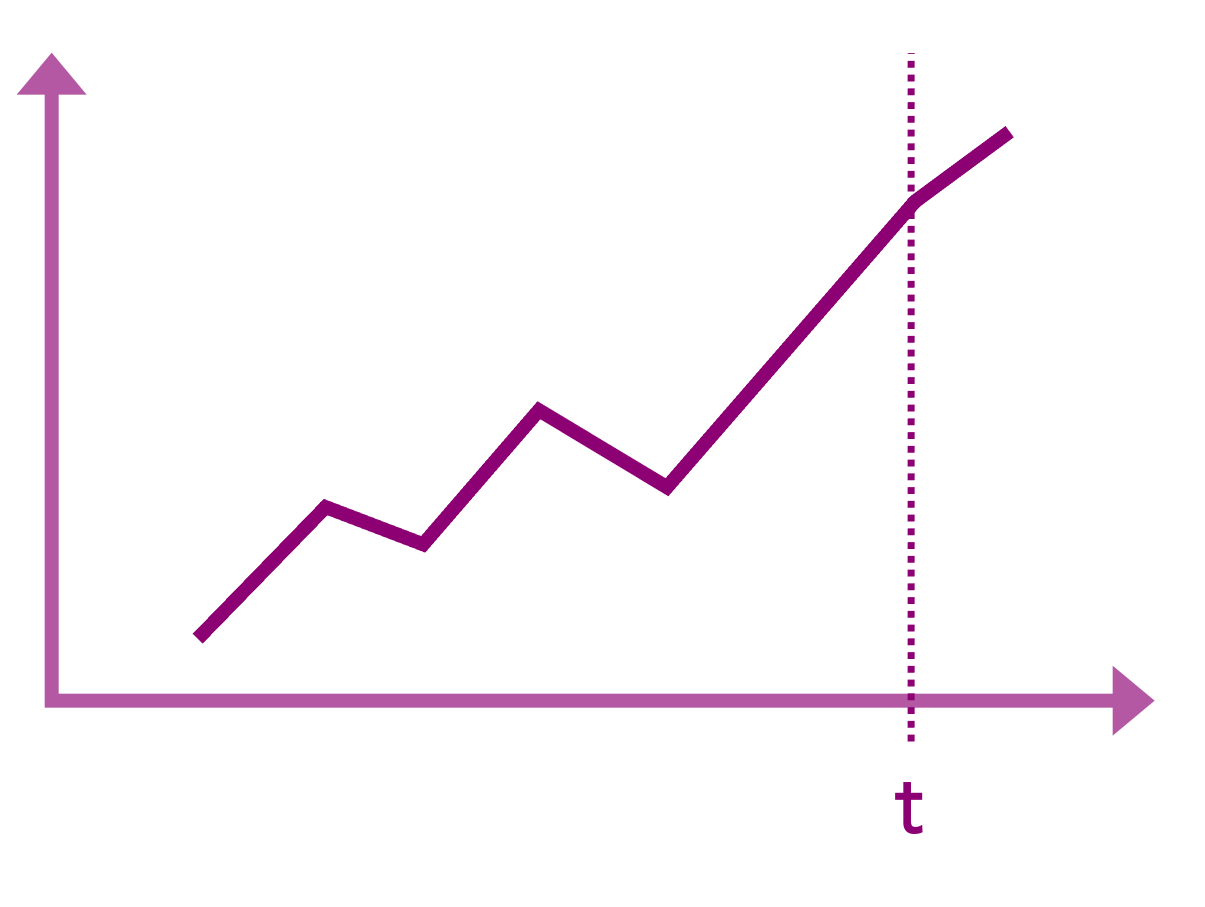
\includegraphics[width=\linewidth]{../5. report/pictures/preproccessing1.png}
        \caption{Archetype}
        \label{fig:preprocessing1}
    \end{subfigure}%
    \begin{subfigure}{.33\linewidth}
        \centering
        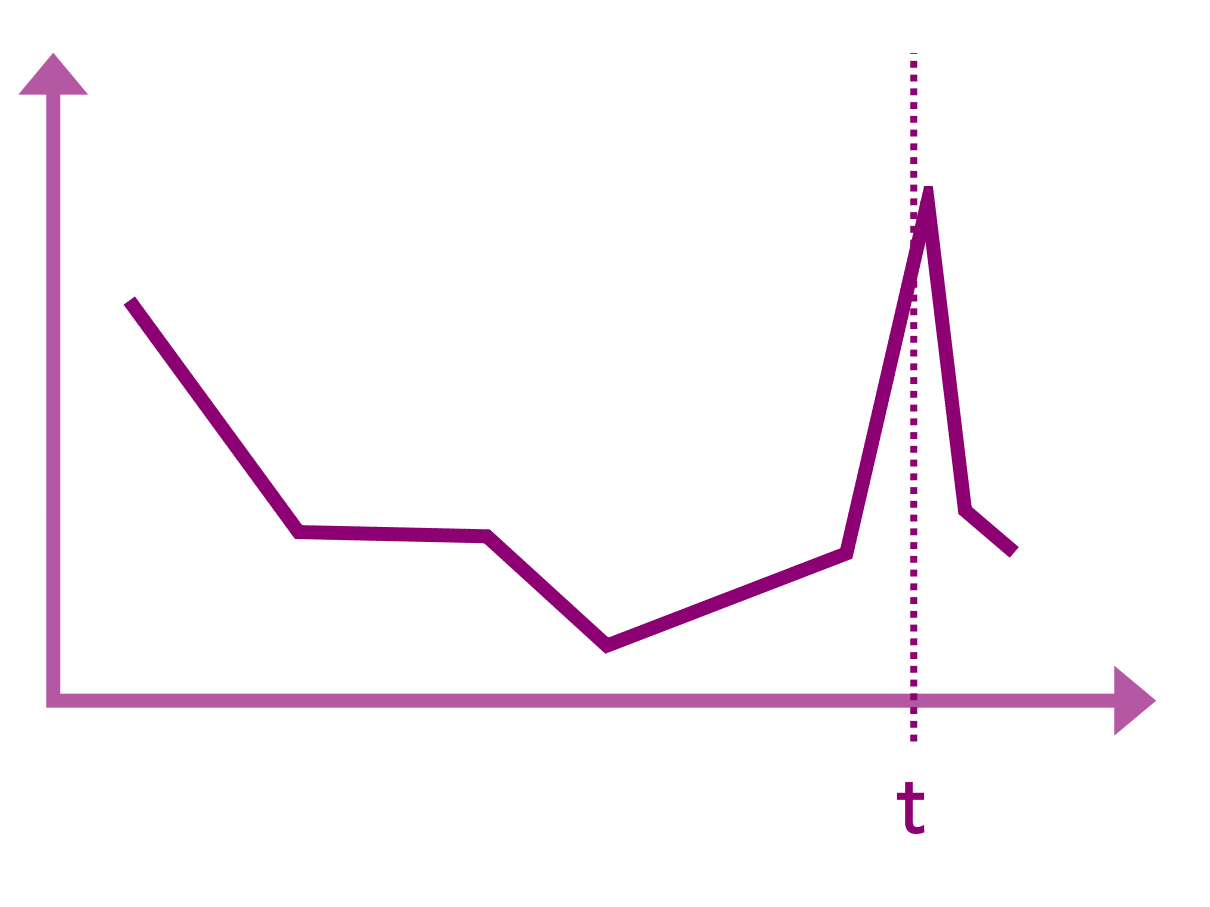
\includegraphics[width=\linewidth]{../5. report/pictures/preproccessing2.png}
        \caption{Pure luck}
        \label{fig:preprocessing2}
    \end{subfigure}%
    \begin{subfigure}{.33\linewidth}
        \centering
        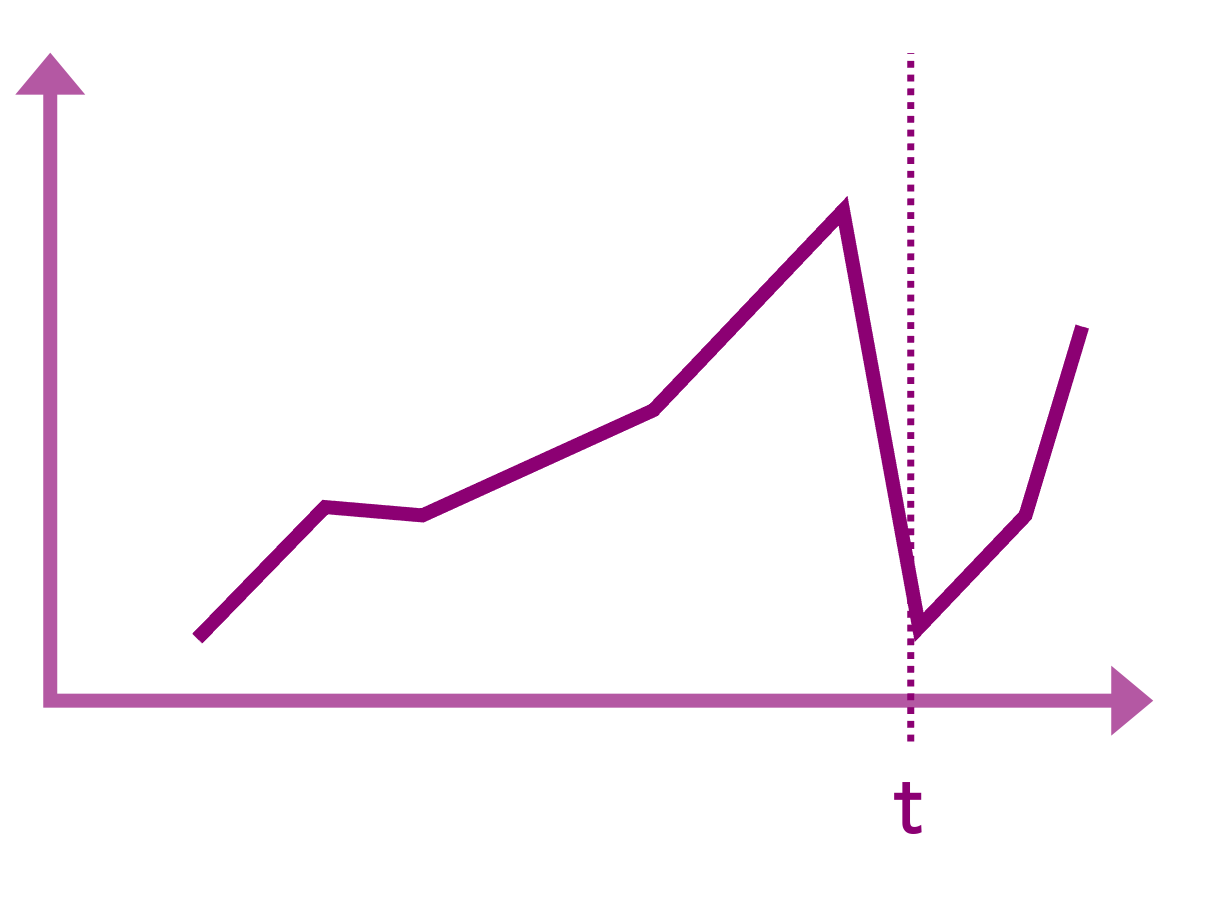
\includegraphics[width=\linewidth]{../5. report/pictures/preproccessing3.png}
        \caption{Bad luck}
        \label{fig:preprocessing3}
    \end{subfigure}
    \caption{Different stock developments as charts: Comparing the archetype of a good investment to spurious spikes (positive and negative). }
    \label{fig:preprocessing}
\end{figure}

The final data (1586 reports) is split into a training, development and test set with a ratio of 70:10:20 (1103, 165, 318). The training set is used to train the models, the development set to optimize the hyperparameters and the test set to evaluate the models.
\section{Foundations} %Mohamad
What are the foundations of our approach? What is the goal? Sentiment Classification.
\subsection{Transformer models}%Mohamad
What are transformer models? 
Build an intuition on self-attention and multi-head attention. 
Use the presentation pictures (youtube video) and reproduce the images quickly in a sketch style on iPad.
\subsection{Parameter efficient fine tuning (PEFT)}%Mohamad
We want to explore many models and fine-tune them on our data. So we need a more efficient approach: PEFT.
What are adapters? Why do we use them? How do we use them?
What is so efficient about it? How does it work?
\cite{Poth2023}

\begin{figure}[h!]
    \centering
    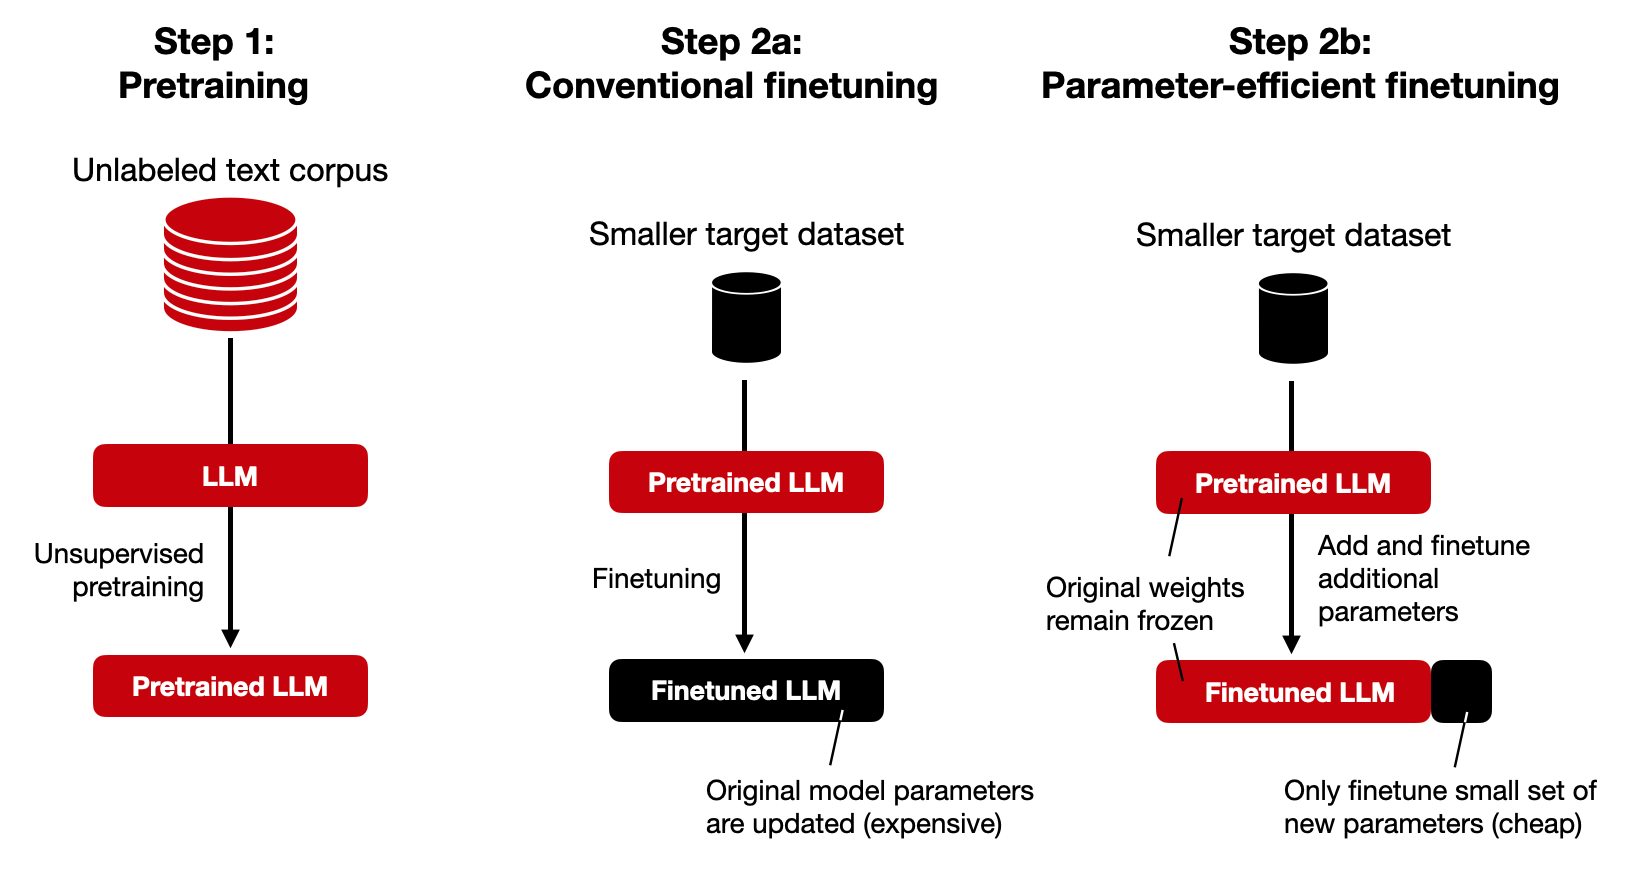
\includegraphics[width=.65\linewidth]{pictures/PEFT1.png}
    \caption[PEFT1]{process of PEFT  \cite{Raschka2023}}
    \label{fig:PEFT1}
\end{figure}

\begin{figure}[h!]
    \centering
    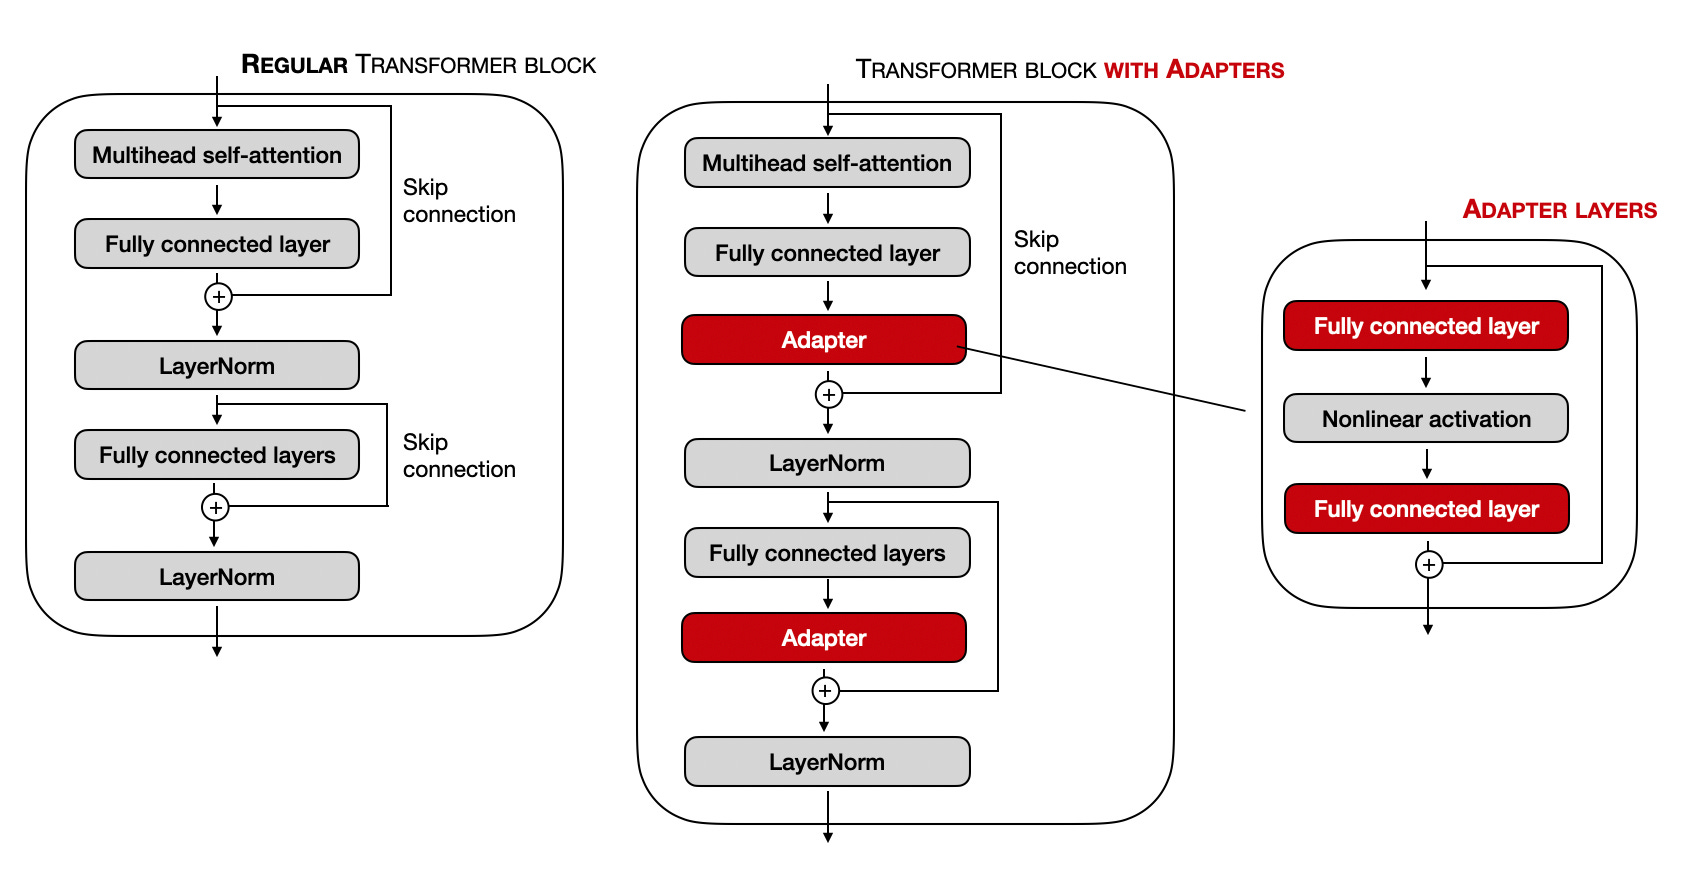
\includegraphics[width=.65\linewidth]{pictures/PEFT2.jpg}
    \caption[PEFT2]{process of PEFT (detailed) \cite{Raschka2023}}
    \label{fig:PEFT2}
\end{figure}   




\subsection{Hugging Face}%Mohamad
What is Hugging Face? Why do we use it? What are the benefits?

\section{literature}%Jonas

As described in \cite{Zhao2024}, there are many different applications of LLMs, and specifically for analyst reports they can provide insights into subtle tone and sentiment to add value. However, at the moment there is only research on publicly available data such as Reddit \cite{Deng2023}. Furthermore, it has been shown that reports may have a small positive performance in the right market conditions \cite{Su2020}, but it is unclear whether only recommendations themselves can influence markets \cite{Brauer2018} and reports have no value at all \cite{Panchenko2007}. Thus, the herding factor may have an impact on stock performance \cite{Palmer2018}.
In \cite{Kim2023} they use LLMs to better interpret and analyze Korean financial analysts' reports.
In this paper, however, we use data from widely spread reports (from retail traders to professionals) on globally traded firms. We show that while analysts can barely outperform the current market, they provide comprehensive textual justifications that enable informed decisions. We use enhanced large language models to efficiently analyze the textual data, allowing a broad exploration of different pre-trained models to identify the subtle underlying sentiment and extract more value from the reports than the experts themselves.


\section{Approach}%Jonas
Our ultimate objective can be interpreted as a binary classification problem based on sentiment analysis. We use the textual data from the reports to predict whether the stock is a good investment or not. In order to do so we compare the performance of different models and configurations to find the best one. We also compare the performance of the models to the analysts' own predictions and other metrics from the report to create a baseline. In order to explore many different models and configurations, we use the parameter efficient fine-tuning approach. We use adapters to fine-tune the models and Hugging Face to access the pre-trained models. Even though literature has shown adapters to be more efficient while retaining the performance of the underlying model, we setup a preliminary experiment with the Stanford Sentiment Treebank v2 (SST2) data set for sentiment classification to validate our approach and compared the efficiency and performance of the models:
% here a table with results for 

\begin{table}[h!]
    \centering
    \begin{tabular}{lcc}
    \toprule
     & \textbf{Fine-tuned LLM} & \textbf{Fine-tuned Adapter} \\ 
     \midrule
    \textbf{Training Runtime} & 1h 58m & \textbf{\textcolor{ForestGreen}{24m}} \\ 
    \textbf{Evaluating Accuracy} & \textbf{\textcolor{ForestGreen}{0.908}} & 0.902 \\
    \textbf{Evaluation Runtime} & 6.83s & \textbf{\textcolor{ForestGreen}{1.84s}} \\ 
    \textbf{Evaluation Loss} & 0.42 & \textbf{\textcolor{ForestGreen}{0.31}} \\ 
    \bottomrule
    \end{tabular}
    \caption{Comparison of Fine-tuned LLM and Fine-tuned Adapter}
    \label{tab:comparison}
    \end{table}


Therefore, we use PEFT to find the best performing setup and built a automated training and evaluation pipeline to efficiently explore the model landscape of Hugging Face.

\subsection{Model selection}%Jonas
Since our approach is centered around sentiment classification of financial reports, we allocated the most fitting pre-trained models from both worlds -- sentiment analysis and finance: 


\noindent
\textbf{Sentiment:}
\begin{itemize}
\item \texttt{kwang123/bert-sentiment-analysis}
\item \texttt{siebert/sentiment-roberta- large-english}
\item \texttt{distilbert/distilbert-base- uncased-finetuned-sst-2-english}
\end{itemize}

\noindent
\textbf{Finance:}
\begin{itemize}
\item \texttt{ProsusAI/finbert}
\item \texttt{yiyanghkust/finbert-tone}
\item \texttt{bardsai/finance-sentiment-pl-fast}
\item \texttt{RashidNLP/Finance-Sentiment- Classification}
\item \texttt{ahmedrachid/FinancialBERT- Sentiment-Analysis}
\item \texttt{soleimanian/financial- roberta-large-sentiment}
\item \texttt{nickmuchi/sec-bert-finetuned- finance-classification}
\item \texttt{nickmuchi/deberta-v3-base- finetuned-finance-text-classification}
\end{itemize}

Among the finance subset, there are also models that are fine-tuned on the task of sentiment classification with finance related text data like the public available SEC filing reports.
\subsection{Adapter configuration}%Mohamad
How can adapters be configured? What are the options? What is the industry standard for our problem and what did we use?
\subsection{Exploration and Exploitation}%Jonas
Since running all possible combinations of configurations is intractable, we assume independence of our various parameters in our experimental setup and base our approach on exploration and exploitation. We explore all possible valid models and configurations and exploit the best ones in the next iteration. First we compare the different models, then we optimise for the best adapter configuration, and after that we search for the best text input. Finally, we compare our PEFT approach to fine-tuning the LLM itself. 
All experiments are performed on the same data, using the same training and test split to ensure comparability, and we use the same evaluation metrics, training parameters and hyperparameters for all models. Everything is run on the same hardware.

\subsection{Evaluation} %Jonas
In order to validate learned models we compare predictions made from the model with previously separated test data. In this way, we can objectively evaluate them according to their predictive qualities. For this comparison, we utilize these fundamental principles:
\newline \textit{Sensitivity} or true positive rate ($\mathrm{TPR}$) is derived from the true positives $\mathrm{TP}$,  i.e., the correctly identified positives $\mathrm{P}$ from the test set: 
$
\mathrm{TPR}=\frac{\mathrm{TP}}{\mathrm{P}}
$
\newline \textit{Specificity} or true negative rate ($\mathrm{TNR}$) is derived from the true negatives $\mathrm{TN}$,  i.e., the correctly identified negatives $\mathrm{N}$ from the test set: 
$
\mathrm{TNR}=\frac{\mathrm{TN}}{\mathrm{N}}
$

\begin{figure}[h!]
    \centering
    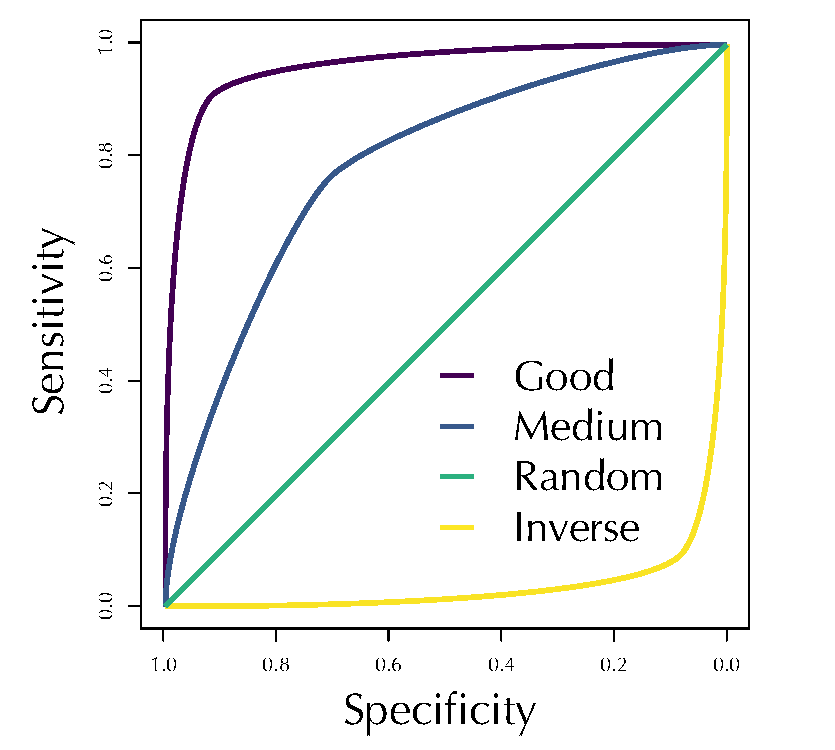
\includegraphics[width=.85\linewidth]{pictures/ROC.pdf}
    \caption[ROC explanation]{Exemplary receiver operating curves for  a \textit{good, medium, random} and \textit{inverse} model fit. The perfect score would be 1.0 on each dimension -- specificity and sensitivity.}
    \label{fig:exroc}
    \end{figure}

By plotting both the sensitivity and specificity in relation for various threshold values, we obtain the so called Receiver Operating Characteristic (ROC) curve. For the results of both measures 1.0 is the optimum, and if the curve is the diagonal, we observed a random process.  In Figure~\ref{fig:exroc}, we can see some common examples of curves. In order to further summarize these evaluations, we can calculate the Area Under the Curve (AUC) to rank the models. Again, a value of 0.5 indicates a random process.  
The reason we use ROC rather than accuracy, precision, recall and f1 score is that ROC is a more comprehensive metric that provides a more detailed view of model performance. In addition, ROC curves make it easier to compare the performance of different models across all classification thresholds. This also makes it more robust to class imbalance, which is very important for inherently unbalanced data such as financial markets, which often follow trends. It also helps to understand how the performance of the model changes with different classification thresholds, which can be crucial for decision making in different conditions where the cost of false positives and false negatives can vary. \cite{Hastie2009}  \cite{Kauermann2021}  \cite{Russell2021}



\section{Results}%Jonas
In this section we present the results of our experiments. We compare the models with classical approaches based on the analysts' forecasts themselves and other metrics from the report to establish a baseline. We present the results of our model training in three steps: First, we compare the different models, then we optimize the best adapter configuration, and finally we search for the text input that provides the highest predictive power. We also directly fine-tune the underlying model to see if PEFT loses significant predictive power. We also use feature attribution via CAPTUM to gain insight into the models and provide an overview of training time, runtime and number of parameters.

\subsection{Benchmarking}%Jonas

We furthermore compare the models with classical approaches based on the analysts forecasts themselves and other metrics from the report to create a baseline.

What are our benchmarks? What are the results?
We use the analysts own predictions as input for a logistic regression model as benchmark.
And we use all the categorical information from the results and yahoo finance as input for a XGBoost random forest model as benchmark.
Results: show \texttt{build\_roc} for n=0 and baseline=True

\subsection{Models in comparison}%Jonas
Discuss results and weather the performance is enough to outperform the analysts.

Show the results of the models.  Show top 5 models and their ROC AUC after initial runs.
First we compare the different models for the same adapter configuration and text input.

\begin{figure}[h!]
    \centering
    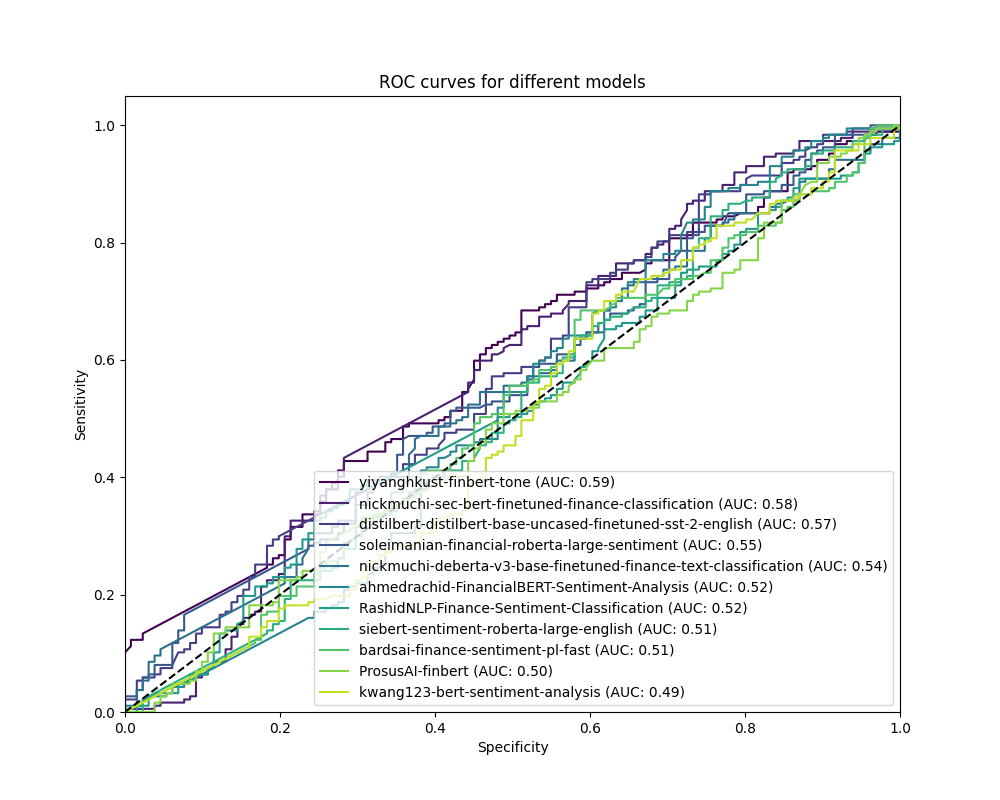
\includegraphics[width=.85\linewidth]{../3. evaluation/roc_curves/First Experiment.png}
    \caption[First Experiment]{First Experiment}
    \label{fig:Firstexp}
\end{figure}


For the best models we then compare the best adapter configurations found in literature:

\begin{figure}[h!]
    \centering
    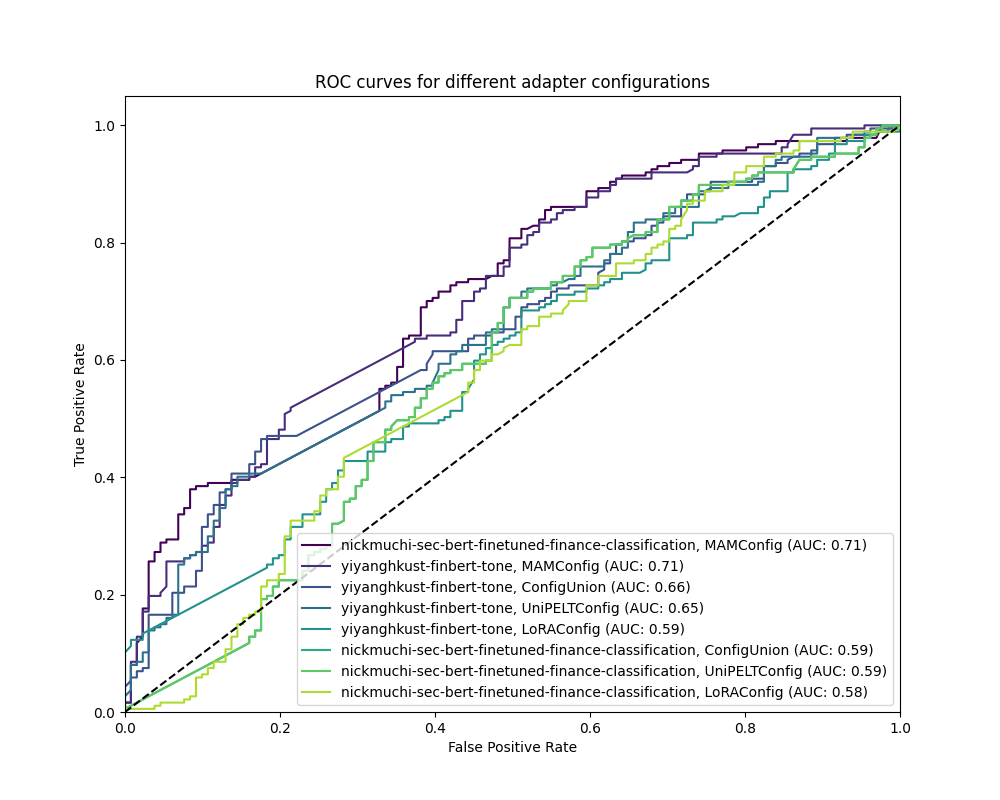
\includegraphics[width=.85\linewidth]{../3. evaluation/roc_curves/Second Experiment.png}
    \caption[Second Experiment]{Second Experiment}
    \label{fig:Secondexp}
\end{figure}

Next to \texttt{AnalystNoteList} we also explore \texttt{BullsList, BearsList, ResearchThesisList, MoatAnalysis, RiskAnalysis, CapitalAllocation, Profile}, and  \texttt{FinancialStrengthText}.

\begin{figure}[h!]
    \centering
    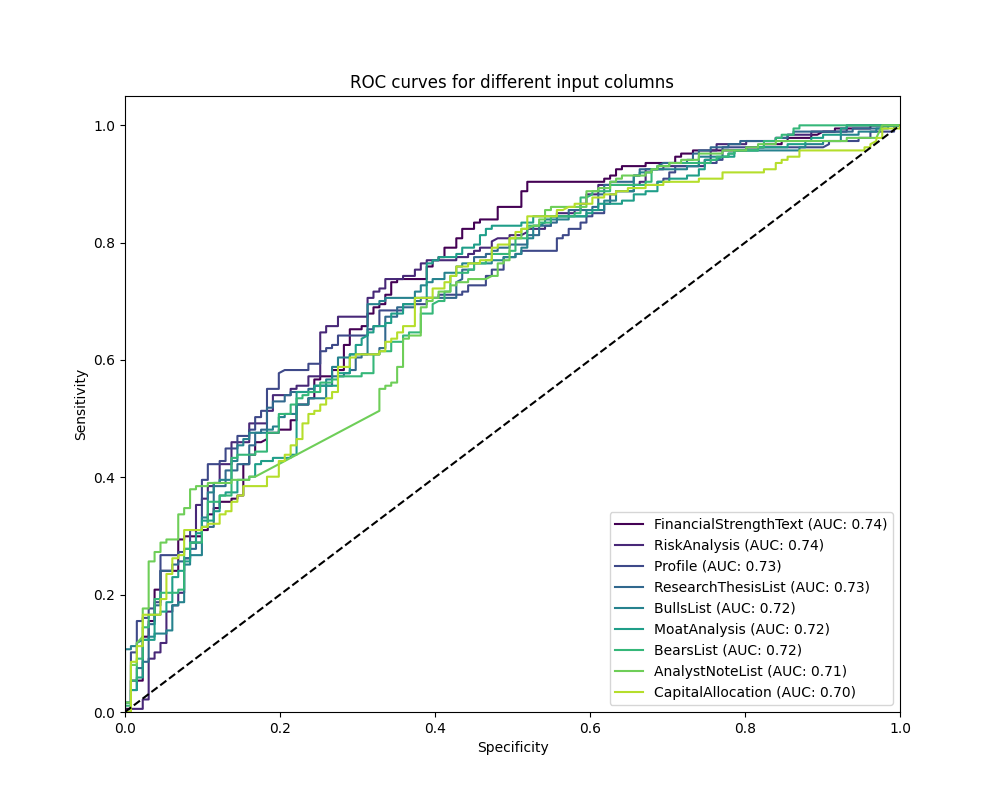
\includegraphics[width=.85\linewidth]{../3. evaluation/roc_curves/Third Experiment.png}
    \caption[Third Experiment]{Third Experiment}
    \label{fig:Thirdexp}
\end{figure}

Finally we use the best found combination to fine-tune the underlying model directly. This only leads to a small improvement of 0.0031 AUC and the training time was the same but the number of parameters could drastically increased from 23 mn to 110 mn.

\begin{figure}[h!]
    \centering
    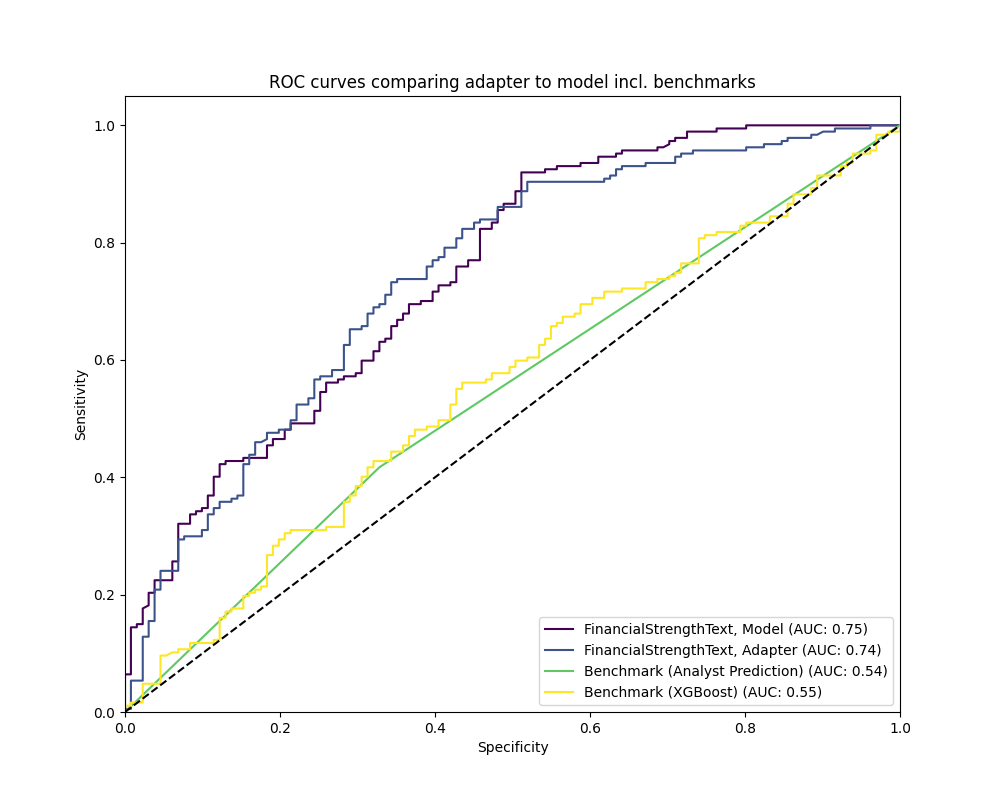
\includegraphics[width=.85\linewidth]{../3. evaluation/roc_curves/Fourth Experiment.png}
    \caption[Fourth Experiment]{Fourth Experiment}
    \label{fig:Fourthexp}
\end{figure}

While there is no overall cutoff value and it highly depends on the specific application, with values above 0.7 \cite{Hosmer2013}, we reached a robust predictive quality.

\subsection{Insights via CAPTUM}%Mohamad
What are the models using as input? Use CAPTUM and quickly describe the gradient approach to obtain feature attribution. \cite{Kokhlikyan2020}


\subsection{Training analysis}%Mohamad
Show some plots about runtime and training time. Compare with Loss, Accuracy etc

\section{Conclusion}
Wrap it up and discuss the results. What are the implications? What are the limitations?
\bibliographystyle{IEEEtran}
\bibliography{report}

\end{document}
